\clearpage





\begin{knitrout}\footnotesize
\definecolor{shadecolor}{rgb}{0.137, 0.137, 0.137}\color{fgcolor}\begin{kframe}
\begin{alltt}
\hlcom{# Data handling}
\hlkwd{library}\hlstd{(dplyr)}
\hlkwd{library}\hlstd{(broom)}
\hlkwd{library}\hlstd{(readxl)}
\hlkwd{library}\hlstd{(sqldf)}

\hlcom{# phylogenetic regression}
\hlkwd{library}\hlstd{(ape)}
\hlkwd{library}\hlstd{(caper)}

\hlcom{# Plotting}
\hlkwd{library}\hlstd{(ggplot2)}
\hlkwd{library}\hlstd{(dotwhisker)}
\hlkwd{library}\hlstd{(ggfortify)}

\hlcom{# Web scraping.}
\hlkwd{library}\hlstd{(rvest)}
\end{alltt}
\end{kframe}
\end{knitrout}

\section{Abstract}


\subsubsection{One or two sentences providing a basic introduction to the field}
% comprehensible to a scientist in any discipline.



\subsubsection{Two to three sentences of more detailed background}
% comprehensible to scientists in related disciplines.


\subsubsection{One sentence clearly stating the general problem (the gap)}
% being addressed by this particular study.


\subsubsection{One sentence summarising the main result}
%  (with the words “here we show” or their equivalent).


\subsubsection{Two or three sentences explaining what the main result reveals in direct comparison to what was thought to be the case previously}
% or how the main result adds to previous knowledge


\subsubsection{One or two sentences to put the results into a more general context.}



\subsubsection{Two or three sentences to provide a broader perspective, }
% readily comprehensible to a scientist in any discipline.



%%%%%%%%%%%%%%%%%%%%%%%%%%%%%%%%%%%%%%%%%%%%%%%%%%%%%%%%%%%%%%%%%%%%%%%%%%%%%%%%%%%%%%%%%%%%%%%%%%%%%%%%%%%%%%%%%%%%%%%%%%%%%%%%%%%%%%%%%%%%%%%%%%%%%%%%%%%

\clearpage
\section{Introduction}

%%%%%%%%%%%%%%%%%%%%%%%%%%%%%%%%%%%%%%%%%%%%%%%%%%%%%%%%%%%%%%%%%%%%%%%%%%%%%%%%%%%%%%%%%%%%%%%%%%%%%%%%%%%%%%%%%%%%%%%%%%%%%%%%%%%%%%%%%%%%%%%%%%%%%%%%%%%





%%%%%%%%%%%%%%%%%%%%%%%%%%%%%%%%%%%%%%%%%%%%%%%%%%%%%%%%%%%%%%%%%%%%%%%%%%%%%%%%%%%%%%%%%%%%%%%%%%%%%%%%%%%%%%%%%%%%%%%%%%%%%%%%%%%%%%%%%%%%%%%%%%%%%%%%%%%

\clearpage
\section{Methods}

%%%%%%%%%%%%%%%%%%%%%%%%%%%%%%%%%%%%%%%%%%%%%%%%%%%%%%%%%%%%%%%%%%%%%%%%%%%%%%%%%%%%%%%%%%%%%%%%%%%%%%%%%%%%%%%%%%%%%%%%%%%%%%%%%%%%%%%%%%%%%%%%%%%%%%%%%%%

To measure pathogen richness I used data from \cite{luis2013comparison}. 
These simply include known infections of a bat species with a pathogen species. 
To control for study bias I collected the number of pubmed citations for each bat species including synonyms from ITIS \cite{itis} via the taxize package \cite{chamberlain2013taxize}.


\begin{knitrout}\footnotesize
\definecolor{shadecolor}{rgb}{0.137, 0.137, 0.137}\color{fgcolor}\begin{kframe}
\begin{alltt}
\hlcom{#read in luis2013virus data}
\hlstd{virus2} \hlkwb{<-} \hlkwd{read.csv}\hlstd{(}\hlstr{'data/Chapter3/luis2013comparison.csv'}\hlstd{,} \hlkwc{stringsAsFactors} \hlstd{=} \hlnum{FALSE}\hlstd{)}


\hlstd{virus2}\hlopt{$}\hlstd{binomial} \hlkwb{<-} \hlkwd{paste}\hlstd{(virus2}\hlopt{$}\hlstd{host.genus, virus2}\hlopt{$}\hlstd{host.species)}
\end{alltt}
\end{kframe}
\end{knitrout}


I used to measures of population structure. 
$F_{ST}$ and the number of subspecies.
The number of of subspecies was counted using the Wilson and Reeder taxonomy \cite{wilson2005mammal}.

\begin{knitrout}\footnotesize
\definecolor{shadecolor}{rgb}{0.137, 0.137, 0.137}\color{fgcolor}\begin{kframe}
\begin{alltt}
\hlstd{tax} \hlkwb{<-} \hlkwd{read.csv}\hlstd{(}\hlstr{'data/Chapter3/msw3-all.csv'}\hlstd{,} \hlkwc{stringsAsFactors} \hlstd{=} \hlnum{FALSE}\hlstd{)}

\hlstd{chir} \hlkwb{<-} \hlstd{tax} \hlopt
          \hlkwd{filter}\hlstd{(Order} \hlopt{==} \hlstr{'CHIROPTERA'}\hlstd{)}

\hlcom{# Save some memory.}
\hlkwd{rm}\hlstd{(tax)}

\hlcom{# Count the number of subspecies each bat species has.}
\hlstd{subs} \hlkwb{<-} \hlkwd{sqldf}\hlstd{(}\hlstr{'
  SELECT Family, Genus, Species, COUNT(Subspecies)
  AS NumberOfSubspecies
  FROM chir
  Where Species <> ""
  GROUP BY Genus, Species
               '}\hlstd{)}



\hlcom{# I think each species has 1 row for species and extra rows for subspecies}
\hlcom{#   Check this is true. }
\hlcom{#   If that is correct, then Species with >1 NumberOfSubspecies should be one less.}

\hlstd{SpeciesRows} \hlkwb{<-} \hlkwd{sqldf}\hlstd{(}\hlstr{'
  SELECT Genus, Species, COUNT(Subspecies)
  AS SpeciesRows
  FROM chir
  WHERE Subspecies == "" AND Species <> ""
  GROUP BY Genus, Species
               '}\hlstd{)}

\hlcom{# }
\hlstd{(SpeciesRows}\hlopt{$}\hlstd{SpeciesRows} \hlopt{!=} \hlnum{1}\hlstd{)} \hlopt \hlstd{sum}
\hlkwd{all}\hlstd{(SpeciesRows}\hlopt{$}\hlstd{SpeciesRows} \hlopt{==} \hlnum{1}\hlstd{)}

\hlcom{# Species with >1 NumberOfSubspecies should be one less}
\hlstd{subs}\hlopt{$}\hlstd{NumberOfSubspecies} \hlkwb{<-} \hlkwd{ifelse}\hlstd{(subs}\hlopt{$}\hlstd{NumberOfSubspecies} \hlopt{>} \hlnum{1}\hlstd{,}
                             \hlstd{subs}\hlopt{$}\hlstd{NumberOfSubspecies} \hlopt{-} \hlnum{1}\hlstd{,}
                             \hlstd{subs}\hlopt{$}\hlstd{NumberOfSubspecies)}

\hlcom{# Quick look at species with highest number of subspecies.}
\hlstd{subs[}\hlkwd{order}\hlstd{(subs}\hlopt{$}\hlstd{NumberOfSubspecies,} \hlkwc{decreasing} \hlstd{=} \hlnum{TRUE} \hlstd{),]} \hlopt \hlstd{head}

\hlcom{# Megaderma spasma is top. It's widespread across south east asia islands. }
\hlcom{#   So this makes sense.}

\hlcom{# Quick look at the number of subspecies.}
\hlkwd{ggplot}\hlstd{(subs,} \hlkwd{aes}\hlstd{(}\hlkwc{x} \hlstd{= NumberOfSubspecies))} \hlopt{+}
  \hlkwd{geom_histogram}\hlstd{()} \hlopt{+}
  \hlkwd{xlab}\hlstd{(}\hlstr{'Number of Subspecies'}\hlstd{)} \hlopt{+}
  \hlkwd{ylab}\hlstd{(}\hlstr{'Count'}\hlstd{)}
\end{alltt}
\end{kframe}\begin{figure}[t]

{\centering 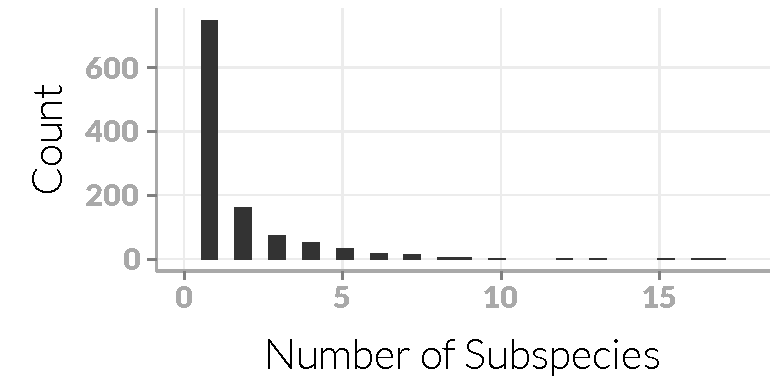
\includegraphics[width=0.8\textwidth]{figure/wilsonReaderTaxonomyRead-1} 

}

\caption[Histogram of number of subspecies]{Histogram of number of subspecies}\label{fig:wilsonReaderTaxonomyRead}
\end{figure}

\begin{kframe}\begin{alltt}
\hlcom{# Create a combined binomial name column}
\hlstd{subs}\hlopt{$}\hlstd{binomial} \hlkwb{<-} \hlkwd{paste}\hlstd{(subs}\hlopt{$}\hlstd{Genus, subs}\hlopt{$}\hlstd{Species)}
\end{alltt}
\end{kframe}
\end{knitrout}

\begin{knitrout}\footnotesize
\definecolor{shadecolor}{rgb}{0.137, 0.137, 0.137}\color{fgcolor}\begin{kframe}
\begin{alltt}
\hlcom{# Compare the histograms of numbers of subspecies over the families with many species.}
\hlstd{subs} \hlopt
  \hlkwd{filter}\hlstd{(Family} \hlopt \hlkwd{names}\hlstd{(}\hlkwd{which}\hlstd{(}\hlkwd{table}\hlstd{(subs}\hlopt{$}\hlstd{Family)} \hlopt{>} \hlnum{99}\hlstd{)))} \hlopt
  \hlkwd{ggplot}\hlstd{(.,} \hlkwd{aes}\hlstd{(}\hlkwc{x} \hlstd{= NumberOfSubspecies,} \hlkwc{y} \hlstd{= ..density..))} \hlopt{+}
    \hlkwd{geom_histogram}\hlstd{()} \hlopt{+}
    \hlkwd{facet_grid}\hlstd{(.} \hlopt{~} \hlstd{Family)} \hlopt{+}
    \hlkwd{xlab}\hlstd{(}\hlstr{'Number of Subspecies'}\hlstd{)} \hlopt{+}
    \hlkwd{ylab}\hlstd{(}\hlstr{'Density'}\hlstd{)}
\end{alltt}
\end{kframe}\begin{figure}[t]

{\centering 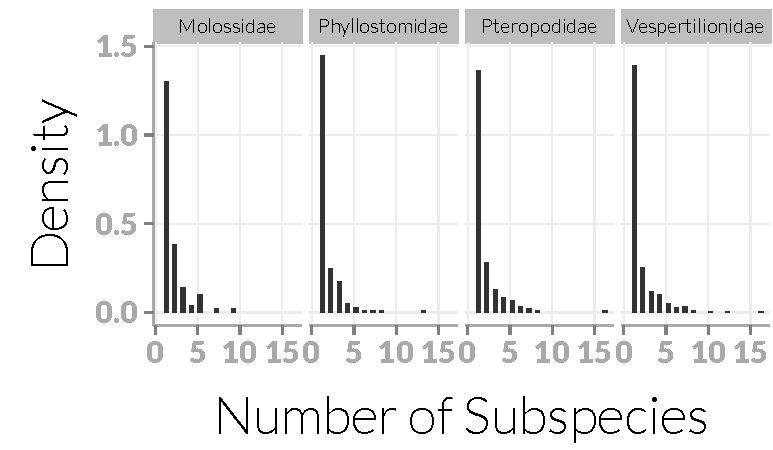
\includegraphics[width=0.8\textwidth]{figure/subsHistsByFam-1} 

}

\caption[Histograms of number of subspecies for the families with many species]{Histograms of number of subspecies for the families with many species.}\label{fig:subsHistsByFam}
\end{figure}


\end{knitrout}

\begin{knitrout}\footnotesize
\definecolor{shadecolor}{rgb}{0.137, 0.137, 0.137}\color{fgcolor}\begin{kframe}
\begin{alltt}
\hlstd{subvsvirus} \hlkwb{<-} \hlstr{'
Number of viruses against number of subspecies.
Points are coloured by family, with families with less than 10 species being grouped into "other".
Contours show the 2D density of points and suggest a positive correlation.
'}
\end{alltt}
\end{kframe}
\end{knitrout}

\begin{knitrout}\footnotesize
\definecolor{shadecolor}{rgb}{0.137, 0.137, 0.137}\color{fgcolor}\begin{kframe}
\begin{alltt}
\hlcom{# create combined dataframe}

\hlcom{# Join dataframes}
\hlstd{species} \hlkwb{<-} \hlkwd{sqldf}\hlstd{(}\hlstr{"
               SELECT subs.binomial, virus2.[virus.species]
               FROM subs
               INNER JOIN virus2
               ON subs.binomial=virus2.binomial;
              "}\hlstd{)}

\hlcom{# Count number of virus species for each bat species}
\hlstd{nSpecies} \hlkwb{<-} \hlstd{species} \hlopt
              \hlstd{unique} \hlopt
              \hlkwd{group_by}\hlstd{(binomial)} \hlopt
              \hlkwd{summarise}\hlstd{(}\hlkwc{virusSpecies} \hlstd{=} \hlkwd{n}\hlstd{())}

\hlcom{# Add other Subspecies data.}
\hlstd{nSpecies} \hlkwb{<-} \hlkwd{sqldf}\hlstd{(}\hlstr{"
              SELECT nSpecies.binomial, virusSpecies, NumberOfSubspecies, Genus, Family
              FROM nSpecies
              LEFT JOIN subs
              ON nSpecies.binomial=subs.binomial
             "}\hlstd{)}

\hlcom{# Create another column to make plotting easier.}
\hlcom{#   Group families with few rows into 'other'}

\hlstd{nSpecies}\hlopt{$}\hlstd{familyPlotCol} \hlkwb{<-} \hlstd{nSpecies}\hlopt{$}\hlstd{Family}
\hlstd{nSpecies}\hlopt{$}\hlstd{familyPlotCol[}
  \hlstd{nSpecies}\hlopt{$}\hlstd{Family} \hlopt \hlkwd{names}\hlstd{(}\hlkwd{which}\hlstd{(}\hlkwd{table}\hlstd{(nSpecies}\hlopt{$}\hlstd{Family)} \hlopt{<} \hlnum{10}\hlstd{))]} \hlkwb{<-} \hlstr{'Other'}

\hlkwd{table}\hlstd{(nSpecies}\hlopt{$}\hlstd{familyPlotCol)}

\hlkwd{ggplot}\hlstd{(nSpecies,} \hlkwd{aes}\hlstd{(}\hlkwc{x} \hlstd{=} \hlkwd{log}\hlstd{(NumberOfSubspecies),} \hlkwc{y} \hlstd{=} \hlkwd{log}\hlstd{(virusSpecies)))}\hlopt{+}
  \hlcom{# geom_smooth(method = 'lm') +}
  \hlkwd{geom_jitter}\hlstd{(}\hlkwd{aes}\hlstd{(}\hlkwc{colour} \hlstd{= familyPlotCol),} \hlkwc{size} \hlstd{=} \hlnum{2.5}\hlstd{,} \hlkwc{alpha} \hlstd{=} \hlnum{0.8}\hlstd{,}
    \hlkwc{position} \hlstd{=} \hlkwd{position_jitter}\hlstd{(}\hlkwc{width} \hlstd{=} \hlnum{.1}\hlstd{,} \hlkwc{height} \hlstd{=} \hlnum{.1}\hlstd{))} \hlopt{+}
  \hlkwd{thesis_palette}\hlstd{()} \hlopt{+}
  \hlkwd{geom_density2d}\hlstd{()} \hlopt{+}
  \hlkwd{labs}\hlstd{(}\hlkwc{colour} \hlstd{=} \hlstr{'Family'}\hlstd{)}
\end{alltt}
\end{kframe}\begin{figure}[t]

{\centering 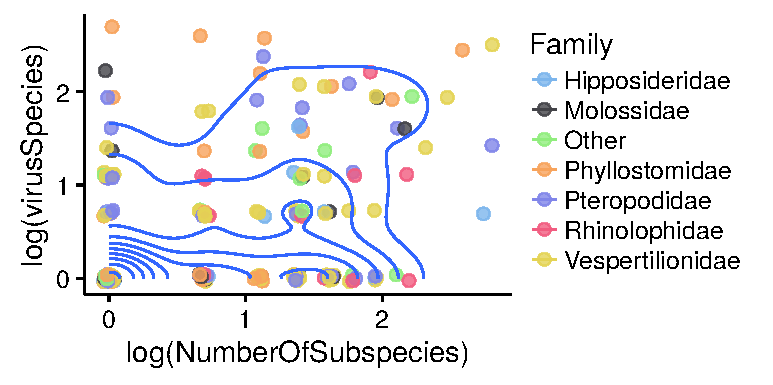
\includegraphics[width=\textwidth]{figure/subsDataFrame-1} 

}

\caption[
Number of viruses against number of subspecies]{
Number of viruses against number of subspecies.
Points are coloured by family, with families with less than 10 species being grouped into "other".
Contours show the 2D density of points and suggest a positive correlation.
}\label{fig:subsDataFrame}
\end{figure}


\end{knitrout}



%%being.rcode euthRead




%%end.rcode






%%%%%%%%%%%%%%%%%%%%%%%%%%%%%%%%%%%%%%%%%%%%%%%%%%%%%%%%%%%%%%%%%%%%%%%%%%%%%%%%%%%%%%%%%%%%%%%%%%%%%%%%%%%%%%%%%%%%%%%%%%%%%%%%%%%%%%%%%%%%%%%%%%%%%%%%%%%

\clearpage
\section{Results}

%%%%%%%%%%%%%%%%%%%%%%%%%%%%%%%%%%%%%%%%%%%%%%%%%%%%%%%%%%%%%%%%%%%%%%%%%%%%%%%%%%%%%%%%%%%%%%%%%%%%%%%%%%%%%%%%%%%%%%%%%%%%%%%%%%%%%%%%%%%%%%%%%%%%%%%%%%%









%%%%%%%%%%%%%%%%%%%%%%%%%%%%%%%%%%%%%%%%%%%%%%%%%%%%%%%%%%%%%%%%%%%%%%%%%%%%%%%%%%%%%%%%%%%%%%%%%%%%%%%%%%%%%%%%%%%%%%%%%%%%%%%%%%%%%%%%%%%%%%%%%%%%%%%%%%%

\clearpage
\section{Discussion}  

%%%%%%%%%%%%%%%%%%%%%%%%%%%%%%%%%%%%%%%%%%%%%%%%%%%%%%%%%%%%%%%%%%%%%%%%%%%%%%%%%%%%%%%%%%%%%%%%%%%%%%%%%%%%%%%%%%%%%%%%%%%%%%%%%%%%%%%%%%%%%%%%%%%%%%%%%%%







